\documentclass{ctexart}

\usepackage{graphicx}
\usepackage{wrapfig}

\title{并行计算技术的现状与未来}
\author{张明昆 2211585}
\date{\today}

\begin{document}
\maketitle
\tableofcontents
\section{引言}
并行计算是一种计算模式,它利用多个处理单元同时执行计算任务,显著提高了计算速度和效率。
这一概念的起源可以追溯到20世纪60年代早期,当时的科学家们开始探索使用多个处理器来解决大规模科学计算问题。
自那以来,随着微电子技术的飞速发展,各种并行处理器和并行计算机系统相继诞生。
并行计算的重要性体现在其对解决大规模、复杂问题的能力上。在天气预报、气候变化模拟、生物信息学、材料科学、大数据分析等领域,传统的串行计算已经无法满足计算需求。
并行计算技术的应用,不仅大大缩短了计算时间,还使得一些以往认为不可能解决的问题变得可行。

调研的目的在于:一方面,通过分析最新的并行计算技术,了解当前并行体系结构的技术水平和发展方向;
另一方面,通过对比不同国家和地区在并行计算领域的发展历程,探讨并行计算技术对国家科技进步和经济发展的重要作用。
\section{当前并行体系结构的概览}
无论是在超级计算机的巨大规模还是个人计算设备的微观层面,并行计算技术都在不断推进计算能力的边界。
接下来,我们将深入到这些技术在各个领域的具体应用和表现,从而更全面地理解并行体系结构的进步与发展趋势。
\subsection{超级计算机}
Frontier: 位于美国橡树岭国家实验室的Frontier超级计算机,是世界上首台达到exaflop(每秒执行一百亿亿次浮点运算)水平的系统。
它结合了高性能的CPU和GPU,为科学研究和模拟提供前所未有的计算能力。
Frontier利用了AMD的Epyc CPU和Radeon Instinct GPU的组合,整套系统包括9,472个CPU和37,888个GPU,总计CPU内核数达606,208个,GPU内核数达8,335,360个。 \cite{choi2022beating}
通过这种CPU和GPU协同工作的并行计算模型,Frontier实现了高效的数据处理和能源利用率,体现了异构并行计算技术的先进性。

Aurora: 位于阿贡国家实验室的Aurora超级计算机,自2023年以来,它一直是全球第二快的超级计算机。预计其性能优化后将超过2ExaFLOPS,成为有史以来最快的计算机。\cite{intel2023datacenter}
Aurora 配备了基于 Sapphire Rapids-SP 系列的 Xeon CPU 和基于 Ponte Vecchio 设计的 GPU,这些高性能处理单元可以提供强大的计算能力,适应各种高性能计算需求。
特别是GPU的大量使用,标志着并行计算中对于特定任务(如图形处理、数据并行任务等)的处理能力的重视。

富岳: 位于日本理化学研究所的富岳超级计算机,是目前世界上性能最强的超级计算机之一。
它采用富士通48核心A64FX SoC,与过往超级计算机大多采用的Intel或AMD的x86、x64主流平台不同。富岳共有158,976个节点,尖峰性能可达到1 exaFLOPS。\cite{fugaku1}

富岳采用了ARM架构的A64FX处理器,特别设计了高效的向量处理单元和高速的互连网络。
这使得富岳在进行大规模并行处理时能够保持高效能效比,展现了面向能效的并行计算设计思想。

神威·太湖之光: 位于中国无锡的神威·太湖之光,是世界上首个使用中国自主研发的处理器的超级计算机。
其主要特点是高能效比,适用于大规模数值模拟、天气预报、生命科学等多个领域。神威·太湖之光使用的是国产的申威26010处理器,
整套系统高达 40,960 个 SW26010处理器,共有 10,649,600 个CPU核心。每个处理器为一个节点单元,一块主板上有两颗处理器,
32块这样的主板组成一架主机,每台主机作为一个“超级节点”,一共有256个这样的超级节点。 \cite{china93petaflop}
基于片上网络的设计,处理单元之间可以高效地通信。
\subsection{CPU技术}
Intel 酷睿14/13系列:代表了Intel在桌面和移动处理器市场的最新进展,采用了先进的制程技术,显著提高了计算性能和能效比。\cite{intelOfficial}
酷睿14/13系列处理器采用了细致的能源管理机制和更高的时钟频率,
通过优化的多核心和超线程技术支持,能够更高效地并行处理多任务,提升了用户的多任务处理能力和应用响应速度。

Intel Sapphire Rapids/Emerald Rapids系列:这些处理器是针对高性能计算和数据中心市场推出的,引入了多核心设计和支持多线程技术,可以在单个芯片上并行执行多个计算任务。
此外,这些处理器集成了先进的内存技术和高速I/O接口,提升了数据处理的能力和效率,特别适用于云计算、大数据分析和人工智能应用。\cite{intelOfficial}

AMD Zen 4架构:通过采用新的制程技术和架构优化,AMD的Zen 4架构在性能和能效比上取得了重大突破。
Zen 4处理器通过提升每个核心的IPC和增加核心数量,进一步加强了CPU的并行处理能力。\cite{amdOfficial}
此外,支持的高速缓存一致性和低延迟的内存访问技术,优化了核心间的数据并行传输,增强了在服务器、桌面和游戏领域的竞争力。

苹果M3系列处理器:在M1和M2系列的基础上,M3系列处理器为苹果设备带来了更高的性能和能效。采用先进的SoC设计,
集成了多核CPU、GPU和AI加速器等处理单元,这些单元可以高效协同工作,执行复杂的并行计算任务。
特别在图形处理和机器学习等领域,M3系列处理器的并行计算能力使苹果产品在性能和能效比上保持领先。
\subsection{GPU技术}
英伟达Ada Lovelace架构:英伟达的Ada Lovelace架构标志着GPU技术的一大进步。
它通过采用新的架构设计和增加计算核心,显著提高了对游戏、专业可视化应用和数据中心中AI计算的支持能力。Ada Lovelace架构能够同时处理成千上万的并行线程,
使其在执行深度学习和科学计算等需要高度并行处理的任务时表现出色。\cite{nvidiaOfficial}

AMD RDNA3架构:AMD的RDNA3架构在提升GPU能效比和性能方面取得了显著成就,尤其是在处理高分辨率游戏和内容创作方面。RDNA3架构通过增加计算单元和优化内部架构,
提高了并行处理图形和计算任务的能力。这一进步不仅增强了游戏体验,也为专业图形和视频处理提供了强大的支持。\cite{amdOfficial}

Intel Ponte Vecchio:作为Intel针对数据中心和高性能计算市场推出的首款GPU,Ponte Vecchio采用了多项创新技术,
包括高带宽内存和高密度计算单元。这些技术的融合,为AI训练和高性能计算领域提供了前所未有的计算能力和数据吞吐率。Ponte Vecchio的设计重点是优化并行处理性能,
使其在处理数据密集型任务时能够展现出卓越的能力。\cite{intelOfficial}
\section{并行体系结构的进步与发展趋势}
\subsection{技术进步}
并行体系结构的进步主要体现在能效比、计算性能和集成度等方面。通过对比不同代的CPU和GPU架构,我们可以明显看到这些进步。

能效比:随着制程技术的进步,例如从14nm到7nm再到5nm甚至更先进的制程,CPU和GPU的能效比得到了显著提高。这意味着在消耗相同电量的情况下,
新一代的处理器能完成更多的计算任务。例如,AMD的Zen 3与Zen 4架构相比,后者在相同功耗下提供更高的性能。

计算性能:新一代的CPU和GPU通过增加核心数、提高时钟速度和优化架构设计,实现了计算性能的大幅提升。例如,苹果M3系列相比M1系列,
在保持能效的同时,性能提升显著,这得益于其更多的处理核心和更高效的架构设计。

集成度:系统级芯片(SoC)的出现,将CPU、GPU、AI加速器等多种处理单元集成在一个芯片上,显著提高了集成度。这不仅减少了芯片间的数据传输延迟,
也提高了整体系统的性能和能效。例如,苹果的M系列处理器就是一个典型的SoC设计,其集成了多种功能,为不同的应用场景提供了强大的并行计算能力。
\subsection{发展趋势}
更高的能效:随着技术的发展,未来的并行体系结构将继续追求更高的能效比。这意味着新一代的处理器将在消耗更少能源的同时,提供更强的计算性能。

AI与传统计算的融合:AI的广泛应用要求处理器具备强大的AI计算能力。因此,未来的并行体系结构将更加注重AI计算与传统计算的融合,通过专门的AI加速器或优化的指令集来提升AI应用的性能和效率。
更高的集成度和系统级优化:随着技术的发展,未来的并行体系结构将实现更高的集成度,通过将CPU、GPU、AI加速器等多种处理单元集成在单一芯片或紧密集成的模块中,来进一步提高系统性能和能效。
同时,系统级优化,如内存访问优化、数据传输优化等,将成为提升性能的关键因素。

异构并行计算模型的普及:为了适应不同计算任务的需求,异构并行计算将成为一种趋势。这种模型结合了CPU、GPU以及其他类型的处理器的优势,能够针对特定任务提供最优的计算资源,从而提高计算效率和性能。

量子计算与并行计算的结合:随着量子计算技术的进步,未来可能会看到量子计算与传统并行计算的结合。量子处理器在特定类型的计算任务上展现出超越传统处理器的性能,
其与传统并行计算技术的结合将开启并行计算的新篇章。
\section{中国与世界的超级计算机发展对比}
\subsection{中国的发展历史}
中国的计算机工业始于20世纪50年代,通过借鉴苏联的技术,于1958年8月1日研发出国内首台数字电子计算机——103机。\cite{103Machine}
随着时间的推移,进入1970年代,中国对超级计算机的需求急剧增加,这主要是由于中长期天气预报、风洞实验模拟、三维地震数据处理以及新武器的开发和航天事业等领域对计算能力提出了更高的要求。

为了满足这些需求,中国开始致力于超级计算机的研发。1983年12月4日,军方主导成功研制出银河一号超级计算机。\cite{GalaxyToTianhe}
随后,银河二号、银河三号、银河四号等系列的银河超级计算机相继问世,使中国成为全球少数几个能够发布5至7天中期数值天气预报的国家之一。
1992年,中国又成功研发了曙光一号超级计算机。随着时间的发展,人们发现向量型计算机由于自身的局限性难以继续发展,因此转向了并行型计算机的研发。
基于这一新方向,中国研发了神威超级计算机及其后续型号神威蓝光超级计算机。\cite{ShenweiBluelight}
2015年,采用全国产CPU的神威·太湖之光超级计算机达成了世界第一的速度成就,并在软件设计方面获得了次年的戈登贝尔奖,成为继美国和日本之后,第一个获此殊荣的国家,打破了长达30年的获奖格局。\cite{SupercomputingAward}

在民间领域,2002年联想集团研发成功的深腾1800型超级计算机及其系列产品标志着中国超级计算机技术的又一重大进步。
同时,深圳大学自主研发的KD系列超级计算机,主要注重于减小体积和降低电力消耗,而非追求最高速度,这种设计使其可能被应用于军舰或飞机等特定领域。
\begin{figure}[h]
    \centering
    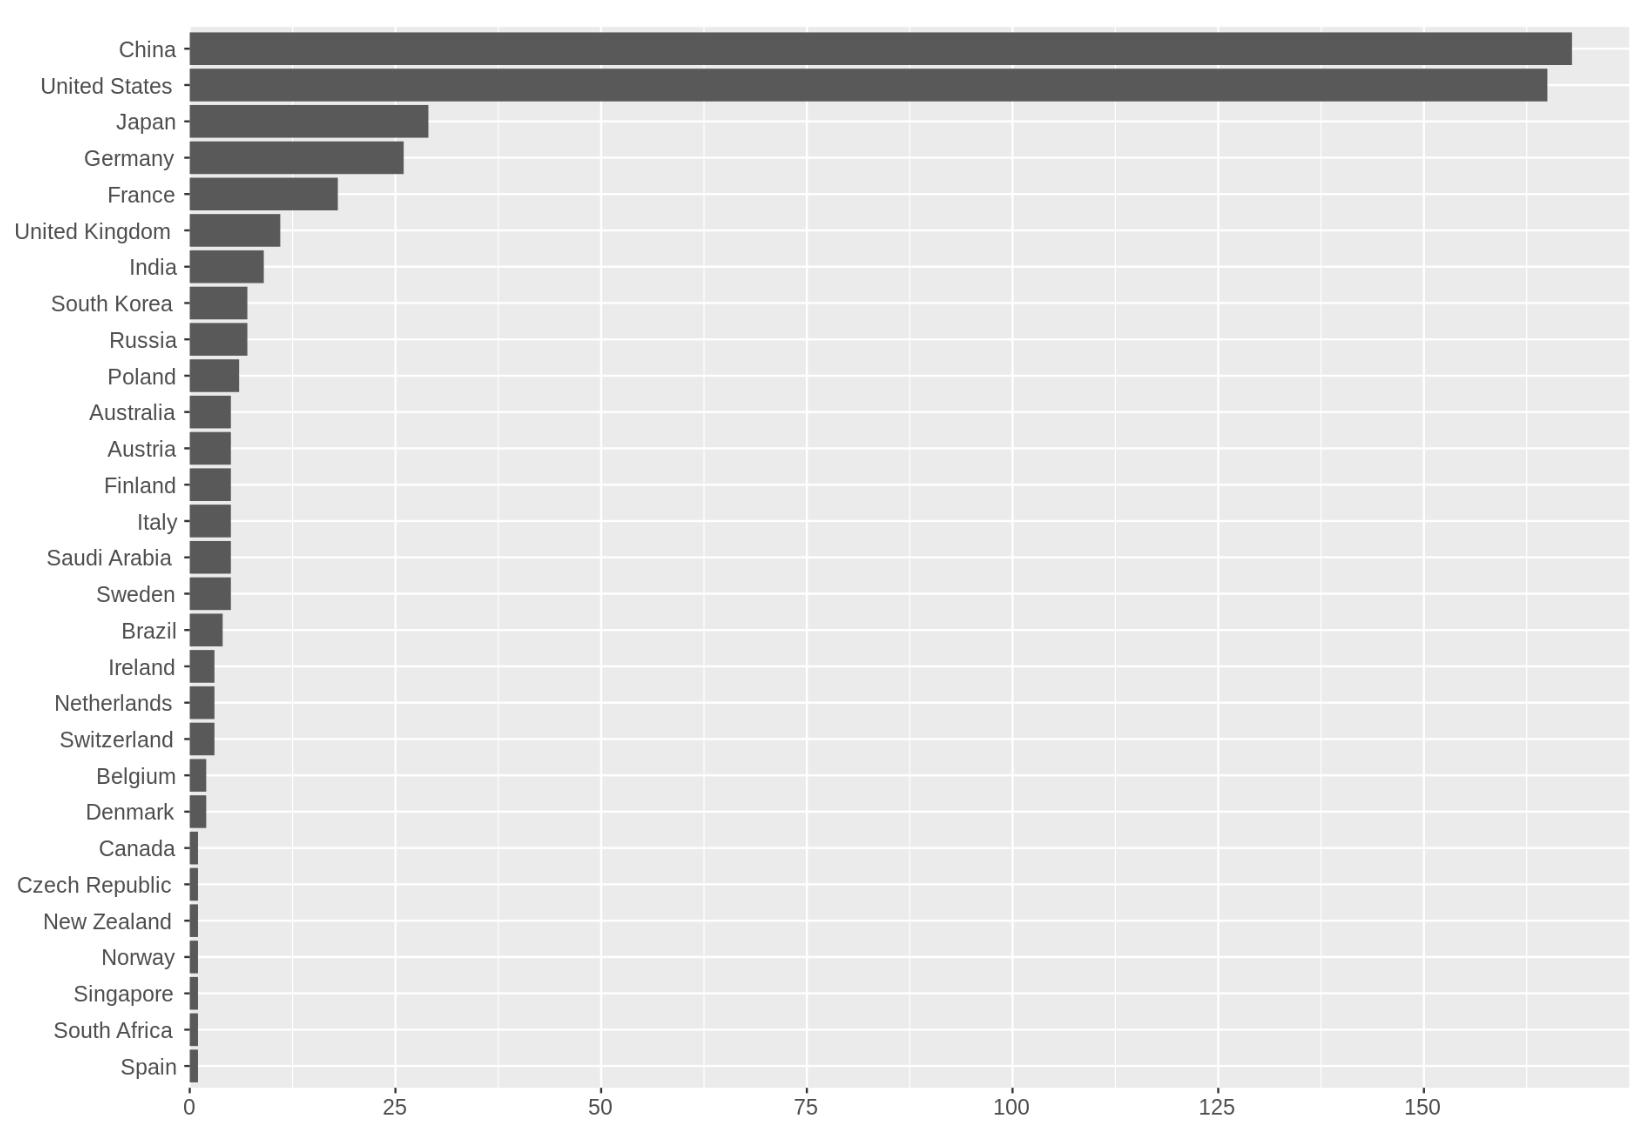
\includegraphics[width=\linewidth]{top500_supercomputers_by_country.png}
    \caption{2016年各国超算算力柱状图}
\end{figure}
\subsection{国际发展历史}
国际上,超级计算机的发展可以追溯到上世纪60年代,美国和欧洲一直是这一领域的领导者。早期的控制数据公司机器可达十倍速于竞争对手,但仍然是比较原始的标量处理器。
到了1970年代,大部分超级计算机就已经是向量处理器了,很多是新进者自行开发的廉价处理器来攻占市场。
1980年代初期,业界开始转向大规模并行计算系统,这时的超级计算机由成千上万的普通处理器所组成。1980年代中叶,将适量的向量处理器(一般由8个到16个不等)联合起来进行并行计算成为通用的方法。
1990年代以后到21世纪初,超级计算机则主要互联基于精简指令集的张量处理器(譬如PowerPC、PA-RISC或DEC Alpha)来进行并行计算。美国的Cray-1(1976年)、日本的富岳(2020年)、
美国的Frontier(2021年)等,都曾是或者是当前世界上最快的超级计算机。
\subsection{重要性与并行体系结构的发展趋势分析}
超级计算机对国家发展的重要性不言而喻,它们在科学研究、国防安全、经济规划和社会管理等多个方面发挥着关键作用。

在气候模拟、生物信息学、材料科学和量子物理等领域,超算是进行高复杂度科学计算和数据密集型研究的关键工具。
它们能够模拟复杂的自然和人工过程,加速新理论和技术的发展,从而推动科学进步和技术创新。

在国防领域,超算用于武器系统设计、加密与解密、战场模拟等关键任务,是维护国家安全的重要资产。通过模拟和分析,超算有助于提升武器性能,优化战略部署,增强防御能力。

并行体系结构是超级计算机发展的核心。随着科技进步,其发展呈现以下趋势:

多核和众核处理器:为了进一步提升计算性能,超算正向着使用更多核心的处理器发展。众核处理器可以处理更多的任务,提高计算效率

异构计算:结合不同类型的处理器(如CPU、GPU和FPGA)进行计算,可以针对不同的计算任务选择最合适的处理器,从而提高效率和能效比

高效能源管理:随着超算性能的提升,能耗问题日益突出。因此,开发高效的能源管理技术,降低功耗,是并行体系结构发展的一个重要方向。

软件和算法的优化:并行计算的软件和算法同样重要,它们需要与硬件发展同步,以充分利用并行体系结构的计算能力。
\begin{thebibliography}{99}
\bibitem{choi2022beating}
Charles Q. Choi, "The Beating Heart of the World's First Exascale Supercomputer," \textit{IEEE Spectrum}, June 24, 2022, archived from the original on August 14, 2022, retrieved August 14, 2022.
\bibitem{intel2023datacenter}
"Intel Data Center GPU Max Series Overview," Intel, retrieved November 14, 2023.
\bibitem{fugaku1}
理化学研究所 计算科学研究センター(R-CCS). スーパーコンピュータ「富岳」プロジェクト. [2019-06-03]. (原始内容存档于2020-05-14) [引用日期: 2019-06-03]. (日语)
\bibitem{china93petaflop}
"China Tops Supercomputer Rankings with New 93-Petaflop Machine." www.top500.org. [2016-06-20]. (原始内容存档于2019-05-31).
\bibitem{intelOfficial}
"Intel Corporation Official Website." www.intel.com. [访问日期: 2024-03-13].
\bibitem{amdOfficial}
"Advanced Micro Devices, Inc Official Website." www.amd.com. [访问日期: 2024-03-13].
\bibitem{nvidiaOfficial}
"NVIDIA Corporation Official Website." www.nvidia.com. [访问日期: 2024-03-13].
\bibitem{103Machine}
中国科学院计算技术研究所. ``103机 - 中国科学院计算研究所官网''. \texttt{http://www.ict.ac.cn/kxcb/kxtp/200909/t20090922\_2514368.html} [2019-05-31]. (页面存档备份,存于互联网档案馆)
\bibitem{GalaxyToTianhe}
``银河到天河 中国超级计算机发展大事记 - IT168网''. \texttt{http://server.it168.com/a2009/1029/800/000000800121.shtml} [2009-10-29]. (页面存档备份,存于互联网档案馆)
\bibitem{ShenweiBluelight}
``全国产化超级计算机神威蓝光问世 耗电量极低 - 东方网''. \texttt{http://mil.eastday.com/m/20111031/u1a6179680.html} [2011-10-31]. (页面存档备份,存于互联网档案馆)
\bibitem{SupercomputingAward}
``Chinese research team wins top award in supercomputing''. [2017-03-10]. (原始内容存档于2016-11-20).
\end{thebibliography}
\end{document}